%\section{Grundlagen zu Threading}


\subsection{Definition von Thread}
Um definieren zu können, was ein Thread ist, müssen zuerst einige weitere Grundbegriffe eingeführt werden. 

Als \emph{Programm} wird in dieser Arbeit die konkrete Niederschrift eines Algorithmus bezeichnet. Die Elemente, aus denen das Programm besteht, werden als \emph{Anweisungen} bezeichnet. Bei der Ausführung eines Programms werden Einzelschritte durchlaufen, diese bezeichnet man als \emph{Aktivitäten}. Eine Sequenz von Aktivitäten, die ein isoliertes Problem abarbeitet, wird \emph{Prozess} genannt. Um diese Definition des Prozessbegriffs von späteren Definitionen abzugrenzen wird er im Folgenden \emph{Rechenprozess} genannt. Die Ausführungseinheit, auf der die Schritte eines Rechenprozesses durchgeführt werden, wird \emph{Prozessor} genannt.\cite{Herrtwich1989}

Wenn ein Programm auf einem Betriebssystem ausgeführt wird, erzeugt das Betriebssystem einen isolierten Adressraum, in dem das Programm ausgeführt wird. Ein Rechenprozess, der auf diese Weise ausgeführt wird, wird als \emph{(System-)Prozess} bezeichnet. Systemprozesse können selbst weitere Systemprozesse starten, wenn das Betriebssystem dies zulässt. Diese Systemprozesse besitzen dann ihren eigenen Adressraum. Die Anzahl der Systemprozesse, die auf einem Rechner laufen, ist meist höher als die Anzahl der Prozessoren des Rechners. Somit können nicht alle Prozesse zur gleichen Zeit laufen. Damit dennoch alle Prozesse voranschreiten können, wechseln moderne Betriebssysteme die Systemprozesse, die auf den Prozessoren des Rechners ausgeführt werden, in schneller Folge. Dabei muss das Betriebssystem einige zu den Systemprozessen gehörende Daten, den \emph{Prozesskontrollblock}, tauschen, sodass der jeweils gerade ausführende Systemprozess seinen eigenen Prozesskontrollblock zur Verfügung hat. Dieser Tausch wird \emph{Kontextwechsel} genannt.\cite{Jobst2018}

Das Speichern und Laden der Prozesskontrollblöcken im Rahmen der Kontextwechsel von Systemprozessen benötigt eine nicht zu vernachlässigende Menge an Zeit. Ein solcher Zeitverbrauch wird auch als \emph{Overhead} bezeichnet. Um den Overhead von Kontextwechseln zu vermindern, bieten moderne Betriebssysteme Systemprozessen die Möglichkeit Rechenprozesse zu erzeugen, die denselben Adressraum wie der erzeugende Systemprozess besitzen. Ein auf diese Art erzeugter Rechenprozess heißt \emph{Thread}. Da die Menge der thread-eigenen Daten, des \emph{Threadkontrollblocks}, deutlich geringer ist als die des Prozesskontrollblocks, erzeugt der Kontextwechsel zwischen Threads einen geringeren Overhead. Zudem können Threads aufgrund des gemeinsamen Adressraums einfacher auf geteilte Ressourcen zugreifen. Das vereinfacht die Kooperation zwischen diesen Rechenprozessen.\cite{Jobst2018}

\subsection{Nebenläufigkeit}\label{sec:nebenl}
Im vorherigen Abschnitt \TODO{hier ist Vergangenheit}{wurde beschrieben}, dass verschiedene Rechenprozesse unabhängig von einander \enquote{gleichzeitig} ablaufen können. Ein Programm wird häufig als \emph{Sequenz} von Anweisungen verstanden. In der Definition von Programm in dieser Arbeit wird bewusst auf das Wort Sequenz verzichtet, denn bei vielen Programmen kann es bei bestimmten Anweisungen irrelevant sein, in welcher Reihenfolge oder ob sie sogar gleichzeitig ausgeführt werden. Man betrachte das folgende Programm in Listing~\ref{lst:squareSeqEx}, das die Quadratsumme zweier Ganzzahlen (im Folgenden auch Quadratsumme genannt) ausgibt: 
\begin{lstlisting}[caption={Beispiel eines Programms das die Summe von Quadraten zweier Ganzzahlen berechnet. Die Berechnung der Quadratzahlen wird nacheinander in einer fest definierten Sequenz durchgeführt.}, label={lst:squareSeqEx}]
printSummedSquare(int a, int b){
  x <- a*a
  y <- b*b
  print(x+y)
}
\end{lstlisting}
Es ist leicht zu erkennen, dass es vollkommen egal ist, ob zuerst \code{x} oder \code{y} ausgerechnet wird oder die Berechnungen simultan stattfinden. Einzig der Ausgabebefehl in Zeile 4 muss ausgeführt werden, nachdem \code{x} und \code{y} berechnet wurden. Zuzulassen, dass die Ausführreihenfolge in dem Programm nicht definiert ist, bringt das Design des Programs näher an die Problembeschreibung \enquote{gib die Quadratsumme zweier Ganzzahlen aus} und ermöglicht auch eine potenziell schnellere Berechnung, da die Quadrate gleichzeitig berechnet werden können.

Paare oder Gruppen von Anweisungen, die (wie Zeile 2 und Zeile 3 des obigen Programms) gleichzeitig oder in beliebiger Reihenfolge ausgeführt werden können, heißen \emph{nebenläufig}. Eine Anweisung kann beispielsweise durch einen Compiler in mehrere Anweisungen geteilt werden oder schon aus mehreren Anweisungen bestehen (man denke zum Beispiel an Funktionsaufrufe). Solche Anweisungen werden \gls{na} genannt. Eine Menge von nebenläufigen Anweisungen, von denen mindestens eine \gls{na} ist, kann \emph{verzahnt} ausgeführt werden. Eine Ausführung von Anweisungen ist verzahnt, wenn zwischen der Ausführung der Teile einer \glsuseri{na} Anweisung andere Anweisungen ausgeführt werden. Abbildung \ref{fig:concAnweisungen} zeigt zur Veranschaulichung die verschiedenen Möglichkeiten, wie zwei nebenläufige \glspl{na} Anweisungen im Zeitverlauf ausgeführt werden können, sowohl auf einem Prozessor als auch auf zwei Prozessoren. 
\begin{figure}[hbt]
\newlength\aOne
\newlength\aTwo
\newlength\aThree
\newlength\bOne
\newlength\bTwo
\pgfmathsetlength{\aOne}{4cm}
\pgfmathsetlength{\aTwo}{2cm}
\pgfmathsetlength{\aThree}{3cm}
\pgfmathsetlength{\bOne}{2.5cm}
\pgfmathsetlength{\bTwo}{3.7cm}
\begin{subfigure}{\textwidth}
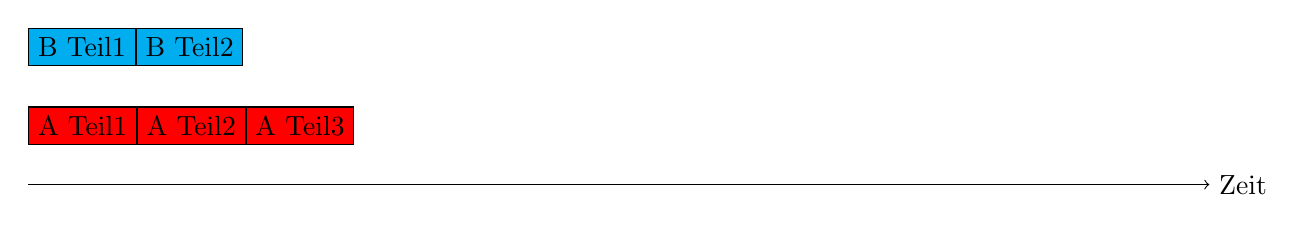
\begin{tikzpicture}

	\draw[->] (0,0) -- (15,0) node[right] {Zeit};
	
	\node[draw,fill=red, anchor=south west, minimum width = \aOne] at (0, .5) (A1) {A Teil1};
	\node[draw,fill=red, anchor=west, minimum width = \aTwo] at (A1.east) (A2) {A Teil2};
	\node[draw,fill=red, anchor=west, minimum width = \aThree] at (A2.east) (A3) {A Teil3};
	
	\node[draw,fill=cyan, anchor=south west, minimum width = \bOne] at (0, 1.5) (B1) {B Teil1};
	\node[draw,fill=cyan, anchor=west, minimum width = \bTwo] at (B1.east) (B2) {B Teil2};

\end{tikzpicture}
\subcaption{Gleichzeitige Ausführung der Anweisungen A und B auf zwei Prozessoren}
\end{subfigure}
\\[1.5em]
\begin{subfigure}{\textwidth}
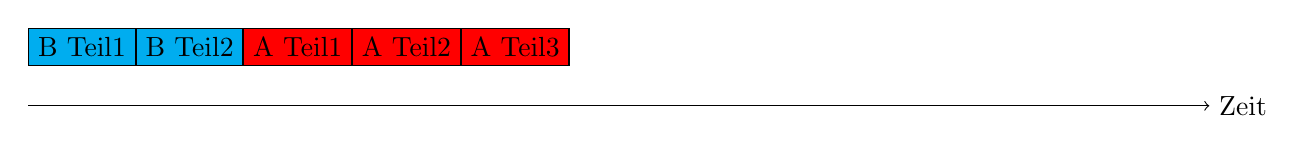
\begin{tikzpicture}

	\draw[->] (0,0) -- (15,0) node[right] {Zeit};
	
	\node[draw,fill=cyan, anchor=south west, minimum width = \bOne] at (0, .5) (B1) {B Teil1};
	\node[draw,fill=cyan, anchor=west, minimum width = \bTwo] at (B1.east) (B2) {B Teil2};
	\node[draw,fill=red, anchor=west, minimum width = \aOne] at (B2.east) (A1) {A Teil1};
	\node[draw,fill=red, anchor=west, minimum width = \aTwo] at (A1.east) (A2) {A Teil2};
	\node[draw,fill=red, anchor=west, minimum width = \aThree] at (A2.east) (A3) {A Teil3};
\end{tikzpicture}
\subcaption{Sequenzielle Ausführung der Anweisungen A und B auf einem Prozessor}
\end{subfigure}
\\[1.5em]
\begin{subfigure}{\textwidth}
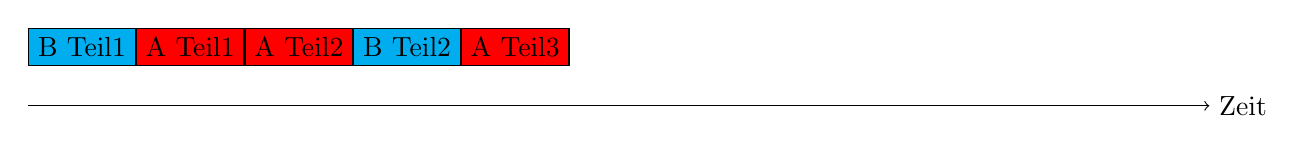
\begin{tikzpicture}

	\draw[->] (0,0) -- (15,0) node[right] {Zeit};
	
	\node[draw,fill=cyan, anchor=south west, minimum width = \bOne] at (0, .5) (B1) {B Teil1};
	\node[draw,fill=red, anchor=west, minimum width = \aOne] at (B1.east) (A1) {A Teil1};
	\node[draw,fill=red, anchor=west, minimum width = \aTwo] at (A1.east) (A2) {A Teil2};
	\node[draw,fill=cyan, anchor=west, minimum width = \bTwo] at (A2.east) (B2) {B Teil2};
	\node[draw,fill=red, anchor=west, minimum width = \aThree] at (B2.east) (A3) {A Teil3};

\end{tikzpicture}
\subcaption{Verzahnte Ausführung der Anweisungen A und B auf einem Prozessor}
\end{subfigure}

\caption{Mögliche Ausführungen nebenläufiger Anweisungen}\label{fig:concAnweisungen}
\end{figure}

Eine der obigen Problemstellung nähere Implementierung der Quadratsumme könnte unter Nutzung von Nebenläufigkeit wie Listing~\ref{lst:squareConcEx} aussehen, dabei wird auf die Schreibweise von \textcite{Herrtwich1989} zurückgegriffen:
\begin{lstlisting}[caption={Beispiel eines Programms mit nebenläufigem Code in einem \code{conc}-Block. Das Programm gibt die Summe von zwei Quadratzahlen aus, wobei die Berechnung der Quadratzahlen nebenläufig stattfindet.}, label={lst:squareConcEx}]
printSummedSquare(int a, int b){
  conc 
    x <- a*a ||
    y <- b*b
  conc end
  print(x+y)
}
\end{lstlisting}
In einem \code{conc}-Block, definiert durch \code{conc} und \code{conc end}, sind alle Anweisungen die durch \code{||} getrennt sind als nebenläufig zu verstehen. Wie man an obigem Beispiel erkennen kann, beschäftigt Nebenläufigkeit sich besonders mit der Struktur und der Möglichkeit der Zusammensetzung voneinander unabhängiger Anweisungen. Somit ist es Aufgabe der nebenläufigen Programmierung, Probleme oder Aufgaben in unabhängige Teile zu zerlegen und zu strukturieren~\cite{Pike2012,Hettel2016}. Blöcke von Anweisungen, die (bezüglich der Aufgabe) nebenläufig sein könnten, aber als Anweisungssequenz definiert sind, werden in dieser Arbeit als \TODO{Hier könnte Prof Kern fragen: Warum?}{\emph{pseudo-sequenzialisiert} bezeichnet}. 

\subsection{Unterschied zwischen Nebenläufigkeit und Parallelität}

\subsection{Folgen von Nebenläufigkeit}
Wie in Abschnitt \ref{sec:nebenl} beschrieben, muss ein Programm keine Sequenz von Anweisungen sein sondern kann auch nebenläufige Anweisungen enthalten. Diese Möglichkeit hat eine Reihe von Folgen, die es bei der nebneläufigen Programmierung zu beachten gilt.
\paragraph{Nichtdeterminismus}
Enthält ein Programm nebenläufige Anweisungen, ist die Reihenfolge der daraus resultierenden Aktivitäten nicht definiert und kann sich bei jedem Programmdurchlauf ändern. Die Ausführung ist also \emph{nichtdeterministisch}, als direkte Folge der Nebenläufigkeit~\cite{Herrtwich1989}. Erwartet man von einem Programm \emph{Determiniertheit}\footnote{Es kann durchaus sein, dass Determiniertheit in einem Programm nicht gewünscht ist. Man betrachte beispielsweise ein Programm, das einen ech-ten Zufallsgenerator beschreibt. Hier wäre Determiniertheit ein direkter Widerspruch zur Aufgabe des Programms.}, also die Eigenschaft, dass gleiche Eingaben immer zu den gleichen Ausgaben führen, ist Nichtdeterminismus in der Regel zu vermeiden~\cite{Herrtwich1989}. Liefert ein Programm bei jeder beliebigen Ausführreihenfolge das selbe Ergebnis, ist es trotz Nichtdeterminismus weiterhin determiniert, weil die Ausführreihenfolge für das Ergebnis keine Rolle spielt. 
\paragraph{Nichtreproduzierbarkeit}
Da das Wissen und die Kontrolle über die Ausführreihenfolge abgegeben wird, wird die Nachvollziebarkeit des Programmablaufs erschwert~\cite{Herrtwich1989}. Tritt beispielsweise ein Fehler auf, kann im Nachhinein nicht ermittelt werden was die Ausführreihenfolge war, die zu dem Fehler geführt hat. Dasselbe Problem ergibt sich ebenfalls, wenn ein nichtdeterminiertes Programm eine Lösung ausgibt und nachvollzogen werden soll, welche Ausführreihenfolge zu diesem Ergebnis geführt hat. Insbesondere das Testen von Software wird dadurch erschwert, da es unmöglich ist bei jedem Test die selben Bedinungen herzustellen, sodass beispielsweise Tests Fehler nicht verlässlich aufzeigen, weil diese nur bei bestimmten Ausführreihenfolgen auftreten~\cite{Herrtwich1989}. Somit muss ein Test entweder alle möglichen Ausführreihenfolgen simulieren oder es muss anderweitig sichergestellt werden, dass die Ausführreihenfolge der nebenläufigen Anweisungen keine Rolle spielt.
\paragraph{Wettkampfbedingungen}
\TODO{Reccource/Datum definieren*}{Daten} und spielen in Programmen eine zentrale Rolle. Greift eine Gruppe von Anweisungen auf die selben (geteilten) Daten zu, ist die Reihenfolge des Zugriffs, wie alle anderen Aktivitäten, beliebig. Wenn mindestens eine der Anweisungen schreibend auf die geteilten Daten zugreift (diese also verändert), hängt der Zustand der Ausgabe des Programms im Allgemeinen von der Reihenfolge der Ausführung ab. Diese Situation wird \emph{Wettkampfbedinung} (engl. Race Condition) genannt~\cite{Hettel2016}. Erwähnenswert ist hier, dass Wettkampfbedingungen nur auftreten können, wenn die geteilten Daten nebenläufig geändert werden. Ausschließlich lesende Zugriffe sind unkritisch, da die Daten unabhängig von der Ausführreihenfolge immer identisch sind. Wenn Daten von lesenden Anweisungen zu jederzeit in einem Zustand gefunden werden, der korrekt ist, werden sie als \emph{threadsicher} bezeichnet. 

Aufgabe der nebenläufigen Programmierung ist es also, Anweisungen so zu strukturieren, dass alle von nebenläufigen Anweisungen genutzten Daten threadsicher sind oder Daten, die nicht threadsicher sind, explizit synchronisiert werden.

\subsection{Synchronisierung}
Um das Auftreten von Wettkampfbedingungen beim schreibenden Zugriff von nebenläufigen Anweisungen auf geteilte Ressourcen zu vermeiden, muss sichergestellt werden, dass der Endzustand nach der Ausführung der Anweisungen unabhängig von der Ausführreihenfolge der daraus resultierenden Aktivitäten ist. Dieser Vorgang wird Synchronisierung genannt.

\paragraph{Snychronisierungsanforderungen} Nach \textcite{Herrtwich1989} gibt es allgemein zwei Arten von Anforderungen an Synchronisierungmechanismen, je nachdem welche Art von Zugriff auf geteilte Ressourcen stattfindet. Sie unterscheiden dabei zwischen \emph{kausal abhäningen} Relationen und \emph{kausal unabhängigen} Relationen zwischen nebenläufigen Anweisungen. Ist Anweisung $B$ kausal abhängig von Anweisung $A$, so dürfen die Aktivitäten von $B$ erst ausgeführt werden, nachdem die Aktivitäten von $A$ abgeschlossen sind. Man schreibt $ A \to B$\todo{Überlegen wie das mit Nebenläufigkeit zusammenhängt. Insbesondere: Unterschied logische Abhängigkeit/strukturelle Abhängigkeit}. 

\paragraph{Synchronisierungsmethoden} Es gibt mehrere Möglichkeiten, die Synchronisierung zwischen nebenläufigen Anweisungen zu erreichen. \textcite{Michael1996} unterteilen Algorithmen diesbezüglich in zwei Kategorien: \emph{blockende} und \emph{nicht-blockende}. Blockende Synchronisierungsalgorithmen führen laut ihnen möglicherweise dazu, dass Rechenprozesse durch andere Rechenprozesse beliebig lang beim Zugriff auf geteilte Daten aufhalten können. Nicht-blockende Algorithmen dagegen garantieren, dass mindestens einer der beteiligten Rechenprozesse mit einer endlichen Anzahl an Aktivitäten endet.